\chapter{Server design and development}
\label{ch:server}

In this chapter, the general model behind the server will be elaborated. The formal documentation with descriptions of the server classes and their methods can be found on page~\pageref{app:documentation}, which also includes an UML class diagram \cite{uml}. An HTML version is also available on \url{mvdenk.com/thesis/doc/}. The description of the model is divided in generic data entries --- entailing the supplanted data by the developer such as the concept map or test items --- and the user attributes, objects and methods --- entailing user specific data such as birthdate or how often a user responded correctly or incorrectly to a certain instance. Only the conceptually relevant methods will be described below, since this keeps the thesis more accessible for readers not familiar with programming paradigms, and these methods are already described within the documentation. For example, the to\_dict() method is prevalent in a large amount of classes, but merely serves the purpose of converting the class into an object that can be sent over the network connection to and rendered within the client and therefore is not conceptually relevant and is not elaborated.

\section{Generic data entries}

There are four classes of generic data: the concept map (containing nodes and edges), the flashcards, the test items and the questionnaire items.

\subsection{Concept map}

The ConceptMap class is mainly a container class consisting of nodes and edges, and certain useful methods for performing standard queries on the concept map. As described in the general definition of the concept map by \citeA{canas}, a Node object represents a concept, and an Edge object represents a relation between two concepts. The Node and Edge were originally intended to be embedded within the ConceptMap class, however this makes them impossible to refer to by other classes in MongoEngine (used for interacting with the MongoDB database). Furthermore, it could theoretically be possible for certain Nodes to exist in different concept maps. Therefore, they are implemented as separate classes in this server model. The example concept map in figure~\ref{fig:examplemap} is used to demonstrate the different functions in of the class.

\begin{figure}
\centering
    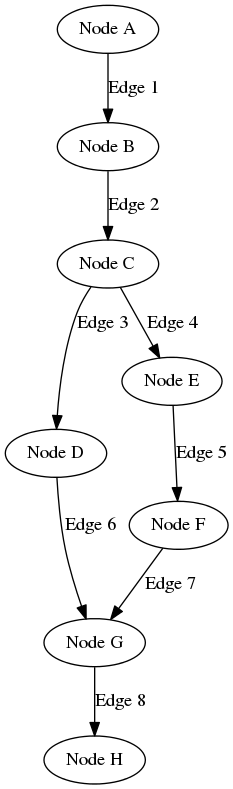
\includegraphics[height=.6\textheight]{img/examplemap.png}
    \caption{An abstract example of a concept map}
    \label{fig:examplemap}
\end{figure}

\paragraph{Nodes} The concepts represented by the nodes are not only an abstract ideas (such as Renaissance Literature), but also more concrete concepts such as a time period (e.g. the Golden Age), a person (e.g. P.C. Hooft) or objects or inventions (e.g. the printing press). Nodes are simple classes only containing a label describing what it should represent and a unique identifyer string.

\paragraph{Edges} An Edge also contains a label describing the specific relation between two concepts and an id, but also contains the references to the id's of the nodes it refers to, one being the `from' node and the other the `to' node, and a list of sources (usually only containing one source), which are the sections of the instructional material the edge is derived from. The model does not make any destinction between a hierarchical and cross-link, since they are the same from a graph rendering perspective. However, this destinction might still be considered for more sophisticated hierarchical rendering or searching algorithms.

Figure~\ref{fig:examplemap_objects} demonstrates how the different classes and attributes represent the concept map from figure~\ref{fig:examplemap}.

\begin{figure}
\centering
    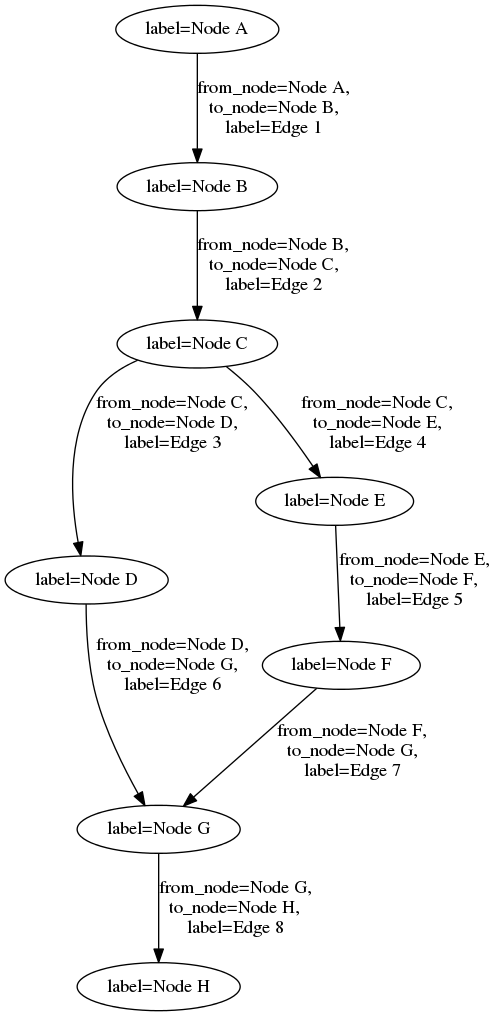
\includegraphics[height=.6\textheight]{img/examplemap_objects.png}
    \caption{The different attributes demonstrated within the example map from figure~\protect\ref{fig:examplemap}}
    \label{fig:examplemap_objects}
\end{figure}

\paragraph{Methods} The most important method of the ConceptMap class is the get\_partial\_map() function, which will provide a new ConceptMap object containing all the parent nodes and edges which directly or indirectly link to a given Node (the parent nodes and edges), plus the nodes and edges linked to by the direct parent nodes (the sibling nodes and edges). This concept map can then be displayed to the user when showing a specific flashmap instance for review. The reason why the parent nodes are returned rather than the child nodes is that in the instructional material the concepts are introduced top-down rather than bottom up, so building up the concept map from parent to child alligns better with the order in which the students read about the concepts. Additionally, the sibling nodes are also returned so that they can be prompted at the same time, and that the user has more context for deciding which concept should be filled in the missing node. Figure~\ref{fig:examplemap_partial_d} and figure~\ref{fig:examplemap_partial_g} demonstrate the get\_partial\_map() function with Node D and Node G from the example map in figure~\ref{fig:examplemap}.

\begin{figure}
\centering
    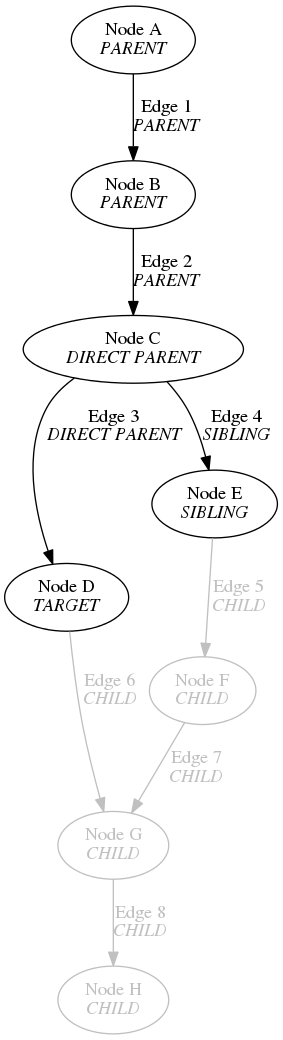
\includegraphics[height=.4\textheight]{img/examplemap_partial_d.png}
    \caption{The result of get\_partial\_map() function with Node D from the example map from figure~\protect\ref{fig:examplemap}}
    \label{fig:examplemap_partial_d}
\end{figure}

\begin{figure}
\centering
    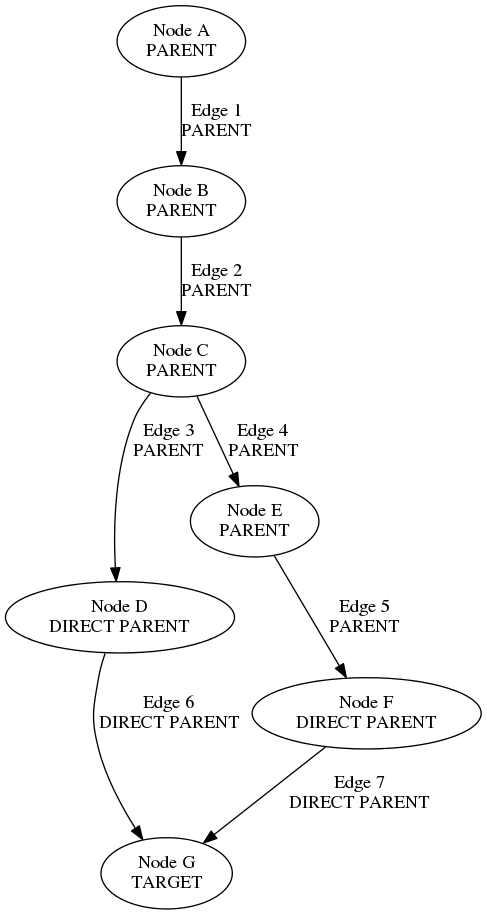
\includegraphics[height=.5\textheight]{img/examplemap_partial_g.png}
    \caption{The result of get\_partial\_map() function with Node G from the example map from figure~\protect\ref{fig:examplemap}}
    \label{fig:examplemap_partial_d}
\end{figure}

\subsection{Flashcards}

A Flashcard class represents a traditional flashcard by simply having a question and answer entry. It addtitionally has an response model entry in order to also function as a test item. In most cases, this is a list only containing the answer entry, however in some cases the answer entry is split into multiple response entries. Finally, since each flashmap is based on the concept map, each Flashcard object also contains a list with Edges the card is derived from. This has the advantage of being able to compare the flashcards with the concept map, but also indirectly relates the flashcards to the sections within the instructional material.

\subsection{Test items}

A TestItem object represents an item on the pre- or posttest. It is very similar to a Flashcard object, with the exception that it directly links to the text sources, and does not contain an answer field since this is never displayed to the user.

\subsection{Questionnaire items}

The QuestionnaireItem class represents items from the Technology Acceptance Model questionnaire \cite{tamq}, and contains a usefulness entry categorising the item as either a Perceived Usefulness item or as a Perceived Ease of Use item, and a positive and a negative phrasing entry. Both phrasings are included instead of only the standard positive phrasing, so that one of these phrasings can be selected when presenting the item to the user, avoiding only one type of phrasing causing a bias within the user towards that specific phrasing.

\section{User attributes, objects and methods}

\subsection{Descriptive attributes}

\subsection{Sessions}

\subsection{Instances}

\begin{figure}
\centering
    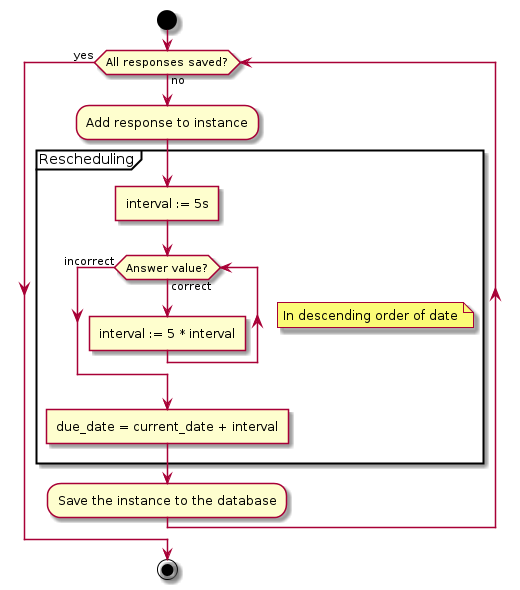
\includegraphics[height=.5\textheight]{img/learningserver.png}
\caption{An UML activity diagram showing the scheduling and saving of a list of responses within instances}
\label{fig:learningserver}
\end{figure}

\subsection{Tests}

\subsection{Questionnaire}
